%%%%%%%%%%%%%%%%%%%%%%%%%%%%%%%%%%%%
%% Template file SP 2024
%% Include in directory homework.sty and headerfooter.tex
%%%%%%%%%%%%%%%%%%%%%%%%%%%%%%%%%%%%

\documentclass[12pt]{article}
\usepackage{homework}
\usepackage{graphicx}
\usepackage{subcaption}
\graphicspath{{images/}}
\geometry{letterpaper, portrait, includeheadfoot=true, hmargin=1in, vmargin=1in}

\setcounter{section}{-1}
%% Solution hiding %%
\usepackage[utf8]{inputenc}
\usepackage{lipsum}


\begin{document}
\singlespacing

\renewcommand{\familydefault}{\rmdefault}
\pagestyle{fancy}
\fancyhf{}
\setlength{\headheight}{30pt}
\renewcommand{\headrulewidth}{0.4pt}
\renewcommand{\footrulewidth}{0.4pt}
\lhead{\large Homework 2 \\ Due Feb. 20, 2024 }
\rhead{\large CS 446 \\ Spring 2024}
\rfoot{\textbf{Page \thepage}}
\lfoot{}

\section{Instructions}

Homework is due Tuesday, April 16, 2024 at 23:59pm Central Time.
Please refer to \url{https://courses.grainger.illinois.edu/cs446/sp2024/homework/hw/index.html} for course policy on homeworks and submission instructions.

\section{GAN: 7pts}
\subsection{}
When G is fixed, the objective function becomes
\begin{align}
&\max_{D}\mathbb{E} _{x\sim p_r(x)}[\log D(x)]+\mathbb{E}_{x\sim p_g(x)}[\log (1-D(x))] \nonumber\\
\Leftrightarrow & \max_{D} \int p_r(x)\log D(x)dx + \int p_g(x)\log (1-D(x))dx \nonumber \\
\Leftrightarrow & \max_{D} \int [p_r(x)\log D(x) + p_g(x)\log (1-D(x))]dx \nonumber
\end{align}
For any given x, we can find a $D^*(x)$ that satisfies
\begin{align}
    D^*(x) = argmax_{D}\{ p_r(x) \log D(x) + p_g(x) \log(1-D(x)) \} \nonumber 
\end{align}
Take derivative to $D$, we get
\begin{align}
    &\frac{p_r(x)}{D^*(x)} - \frac{p_g(x)}{1-D^*(x)} = 0 \nonumber \\
    \Longrightarrow & D^*(x) = \frac{p_r(x)}{p_g(x) + p_r(x)} \label{1.1}
\end{align}

\subsection{}
When D is optimal, put equation (\ref{1.1}) into objective function. We get
\begin{align}
    & \min_{G} \int (p_r \log \frac{p_r}{p_r + p_g} + p_g \log \frac{p_g}{p_r + p_g}) dx \nonumber \\
    =& \min_{G} \int p_r \log p_r dx - \int p_r \log \frac{p_r + p_g}{2}dx - \int p_r \log 2 dx \nonumber \\
     & \quad + \int p_g \log p_g dx - \int p_g \log \frac{p_r + p_g}{2}dx - \int p_g \log 2 dx \nonumber \\
     \Leftrightarrow &  \min_{G} \quad \frac{1}{2} D_{KL}(P_r || \frac{P_r + P_g}{2}) + \frac{1}{2} D_{KL} (P_g || \frac{P_r + P_g}{2}) \nonumber
\end{align}

\subsection{}
When D is perfect, the objective function will consistently equals to 0, which causes the gradients to 0, in other words, the problem of vanishing gradients.

\newpage

\section{Diffusion model : 11pts}
\subsection{}
\begin{align}
    ELBO &= \mathbb{E}_{q_\phi(x_1|x_0)}\log p_\theta(x_0|x_1) - D_{KL}(q_\phi(x_t|x_0) || p_{x_t}) \nonumber \\
    & \quad - \sum_{t=2}^{T}\mathbb{E}_{q_\phi(x_t|x_0)} D_{KL}(q_\phi(x_{t-1}|x_t, x_0) || p_\theta(x_{t-1} | x_t)) \nonumber \\
    & = \sum_{t=1}^{T}\frac{1}{2\sigma_q(t)^2}\frac{\beta_t \bar{\beta}_{t-1}}{(1 - \bar{\beta}_t)^2} \mathbb{E}_{q_\phi(x_t | x_0)} || \hat{x}_\theta(x_t) - x_0 ||^2 \nonumber
\end{align}
Where $\bar{\beta}_t = \Pi_{i=1}^{t}(1-\beta_i)$.
The expectation is with respect to distribution $\mathcal{N}(\sqrt{\bar{\beta}_{t}}x_0, (1 - \bar{\beta}_t)I)$.
\subsection{}
No. The decoder takes input $x_t$ from noise and then generates $x_{t-1}$ from the previous output, and the process goes on. Because don't know the true distribution of each step, we can't directly estimate the density.
But We can estimate it by sampling.

\subsection{}
By using reparameterization trick, we can get 
\begin{align}
    x_1 &= \sqrt{\beta_1}\epsilon_1 + \sqrt{1-\beta_1}x_0 \nonumber \\
    x_2 &= \sqrt{\beta_2}\epsilon_2 + \sqrt{1-\beta_2}x_1 \nonumber \\
    &\quad \vdots \nonumber \\
    x_t &= \sqrt{\beta_t}\epsilon_t + \sqrt{1-\beta_t}x_{t-1} \nonumber
\end{align} Where $\epsilon_i \sim \mathcal{N}(0, I)$.

Put all $x_i$ (i = 1, 2, ..., t-1) into the $x_t$ equation, we get
\begin{eqnarray}
    x_t & = & \sqrt{1 - \beta_t}\sqrt{1 - \beta_{t-1}}\cdots\sqrt{1 - \beta_1}x_0 \nonumber \\
     \quad &+& \sum_{i =  1}^{t-1}\sqrt{1 - \beta_t}\sqrt{1 - \beta_{t-1}}\cdots\sqrt{1 - \beta_{i+1}}\sqrt{\beta_i}\epsilon_i + \sqrt{\beta_t}\epsilon_t \nonumber
\end{eqnarray}
$x_t$ is from a Gaussian distribution with mean $\sqrt{1 - \beta_t}\sqrt{1 - \beta_{t-1}}\cdots\sqrt{1 - \beta_1}x_0$ and variance
\begin{equation}
    \bar{\epsilon}_t = (1 - \beta_t)(1 - \beta_{t-1})\cdots(1 - \beta_2)\beta_1 + (1 - \beta_t)(1 - \beta_{t-1})\cdots(1 - \beta_3)\beta_2 + \cdots + \beta_t \nonumber
\end{equation} 
We can also get variances $\bar{\epsilon}_{t-1}$, $\bar{\epsilon}_{t-2}$, ..., $\bar{\epsilon}_1$ by the same way. We can simplify the equation by using the following equation:
\begin{align}
    & \quad\quad \bar{\epsilon}_{t}  =  (1 - \beta_t)\epsilon_{t-1} + \beta_t \nonumber \\
    &\Leftrightarrow \bar{\epsilon}_{t} - 1  =  (1 - \beta_t)(\epsilon_{t-1} - 1) \nonumber \\
    &\Rightarrow \bar{\epsilon}_{t} - 1  =  -\Pi_{i=1}^{t}(1 - \beta_i) \nonumber \\
    &\Rightarrow \bar{\epsilon}_{t}  =  1 -\Pi_{i=1}^{t}(1 - \beta_i) \nonumber
\end{align}

So, $q(x_t|x_0) = \mathcal{N}(x_t; \Pi_{i=1}^{t}\sqrt{1 - \beta_i}x_0, 1 -\Pi_{i=1}^{t}(1 - \beta_i))  $


\subsection{}
We followed the method from Stanley H. Chan's "Tutorial on Diffusion Models for Imaging and Vision".
\begin{eqnarray}
    q_\phi(x_{t-1} | x_t, x_0) &=& \frac{q_\phi (x_{t-1}, x_t | x_0) }{q_\phi(x_t | x_0)} \nonumber \\
    &=& \frac{q_\phi (x_{t} | x_{t-1}, x_0)q_\phi(x_{t-1} | x_0) }{q_\phi(x_t | x_0)} \nonumber \\
    &=& \frac{\mathcal{N}(x_t|\sqrt{1-\beta _t}x_{t-1}, \beta_tI)\mathcal{N} (x_{t-1}|\sqrt{\bar{\beta}_{t-1}}, (1-\bar{\beta}_{t-1})I)} { N(x_t|\sqrt{\bar{\beta}_{t}}x_0, (1-\bar{\beta}_{t})I)} \nonumber \\
\end{eqnarray}

After calculation of above Gaussian product, we get
\begin{equation}
    q_\phi(x_{t-1} | x_t, x_0) \sim exp{\frac{x_t - \sqrt{1-\beta_t}x_{t-1}}{2\beta_t} + \frac{x_{t-1} - \sqrt{\bar{\beta}_{t-1}x_0}}{2(1-\bar{\beta}_{t-1})} - \frac{x_t - \sqrt{\bar{\beta}_{t}}x_0}{2(1-\bar{\beta}_{t})}} \nonumber 
\end{equation}
Then, we do some variable substitution,
\begin{align}
    x = x_{t}, \quad\quad & a = \sqrt{1-\beta_t} \nonumber \\
    y = x_{t-1}, \quad\quad & b = \sqrt{\bar{\beta}_{t-1}} \nonumber\\
    z = x_0, \quad\quad& c = \sqrt{\bar{\beta}_{t}} \nonumber
\end{align}

Then, we get
\begin{equation}
    f(y) = \frac{x - \sqrt{a}y}{2(1-a)} + \frac{y - \sqrt{b}z}{2(1-b)} - \frac{x - \sqrt{c}z}{2(1-c)} \nonumber
\end{equation}

The mean of $q_\phi(x_{t-1} | x_t, x_0)$ is where the derivative of $f(y)$ equals to 0,
\begin{equation}
    f'(y) = \frac{1-ab}{(1-a)(1-b)}y - (\frac{\sqrt{a}}{1-a}x + \frac{\sqrt{b}}{1-b}z) = 0 \nonumber
\end{equation}
which yeilds
\begin{equation}
    y = \frac{(1-b)\sqrt{a}}{1-ab}x + \frac{(1-a)\sqrt{b}}{1-ab}z \nonumber
\end{equation}

So, the mean of $q_\phi(x_{t-1} | x_t, x_0)$ is,
\begin{equation}
    \mu_q(x_t, x_0) = \frac{(1-\bar{\beta}_{t-1})\sqrt{1 - \beta_t}}{1 - \bar{\beta}_t}x_t + \frac{\beta_t \sqrt{\bar{\beta}_{t-1}}}{1-\bar{\beta}_t}x_0 \nonumber
\end{equation}
where $\bar{\beta}_t = \Pi_{i=1}^{t}(1-\beta_i)$.

\subsection{}
\begin{eqnarray}
    s_\theta(x, \delta | x_{known}) & = & \nabla_{x} \log p_\theta(x , \delta | x_{known}) \nonumber \\
    & = & \nabla_{x} \log \frac{p(x_{known}|x) p_\theta(x, \delta)}{p(x_{known})} \nonumber \\
    & = & \nabla_{x}[\log p(x_{known}|x) + \log p_\theta(x, \delta) - \log p(x_{known})] \nonumber \\
    & = & \nabla_{x}[-||(x - x_{known}) \odot M ||^2] + s_\theta(x, \delta) \nonumber \\
    & = & -2((x - x_{known}) \odot M )+ s_\theta(x, \delta) \nonumber
\end{eqnarray}

\newpage

\section{Unsupervised learning / contrastive learining: 4 pts}
\subsection{}
True.
\subsection{}
False. MAE uses different mask-out rates during training.
\subsection{}
True.
\subsection{}
False. When using CLIP to clssify images, we can insert labels into appropriate sentences for feature extraction, compared with the features of images. If the similarity is high, it can be considered that the labels contained in the sentence are the labels of the image.
\newpage

\section{Coding: GAN, 10pts}

\begin{figure}[H]
    \centering
    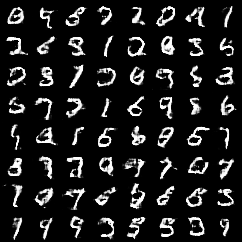
\includegraphics[width=0.5\textwidth]{codes/imgs/gan/test_90.png}
    \caption{Generated images after 90 epochs}
    \label{fig:gan}
\end{figure}


\newpage

\section{Coding: Diffusion model, 10pts}
\begin{figure}[H]
    \centering
    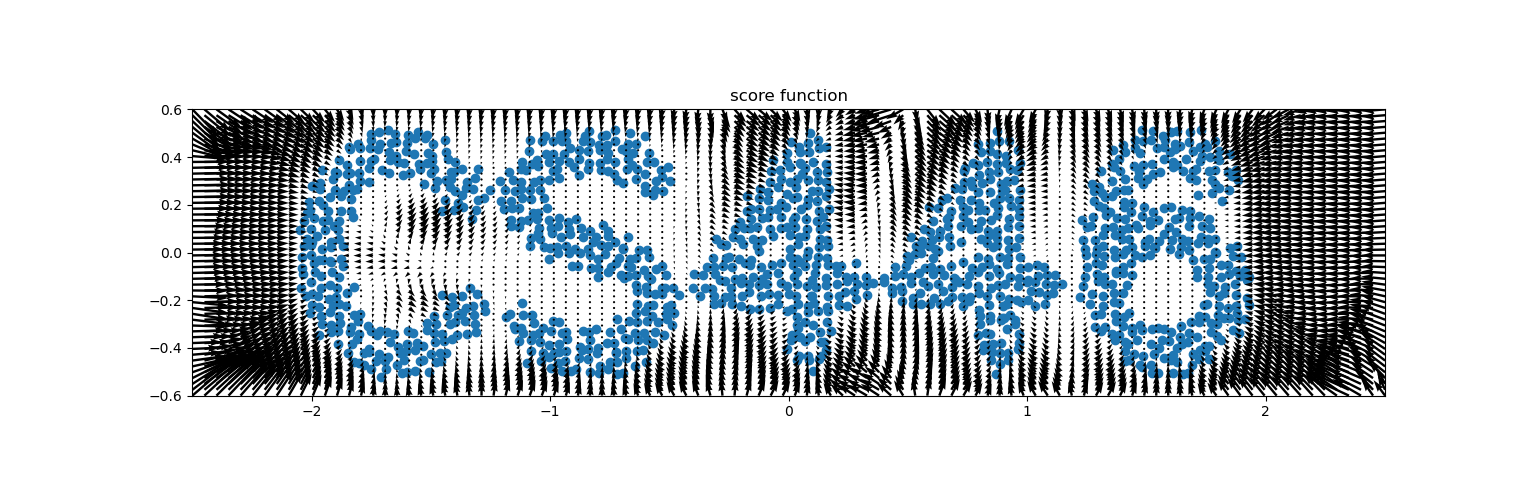
\includegraphics[width=0.5\textwidth]{codes/imgs/diffusion/score_function.png}
    \caption{Score function}
    \label{fig:score}
\end{figure}

\begin{figure}[H]
    \centering
    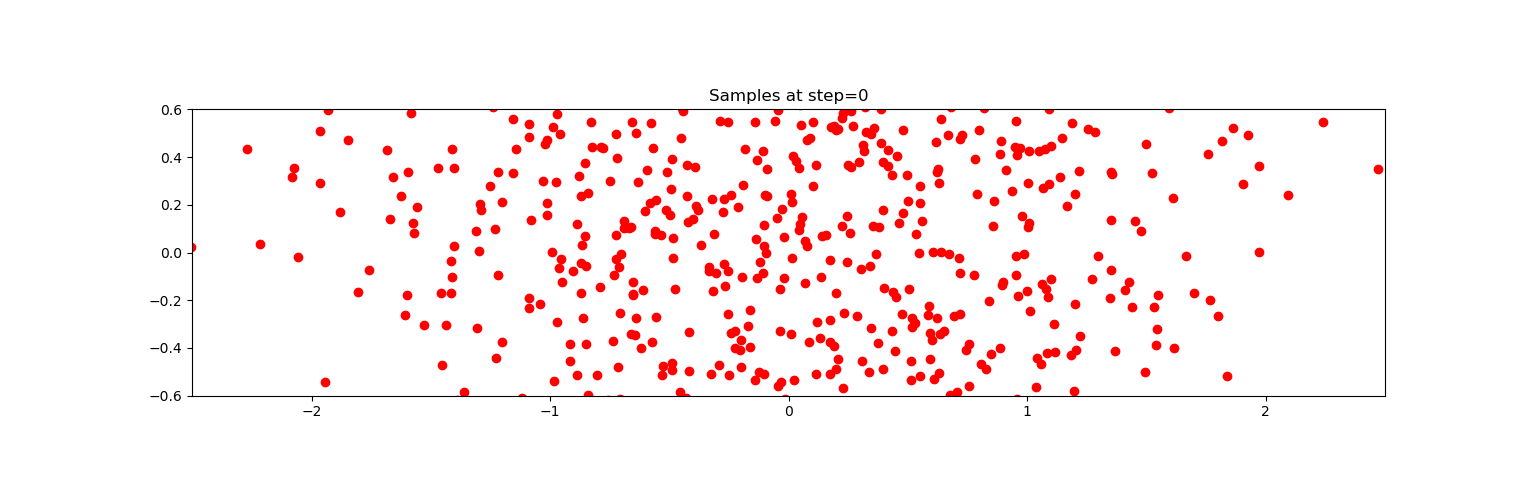
\includegraphics[width=\linewidth]{codes/imgs/diffusion/step0.png}
    \caption{Step 0}
    \label{fig:step0}
\end{figure}

\begin{figure}[H]
    \centering
    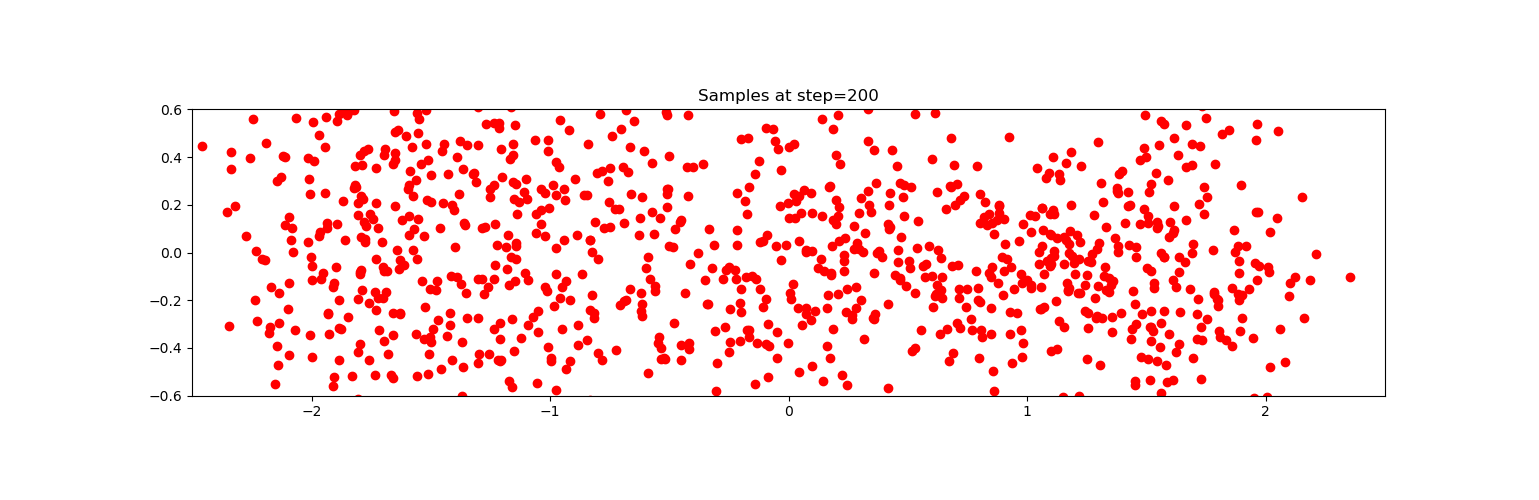
\includegraphics[width=\linewidth]{codes/imgs/diffusion/step200.png}
    \caption{Step 200}
    \label{fig:step200}
\end{figure}

\begin{figure}[H]
    \centering
    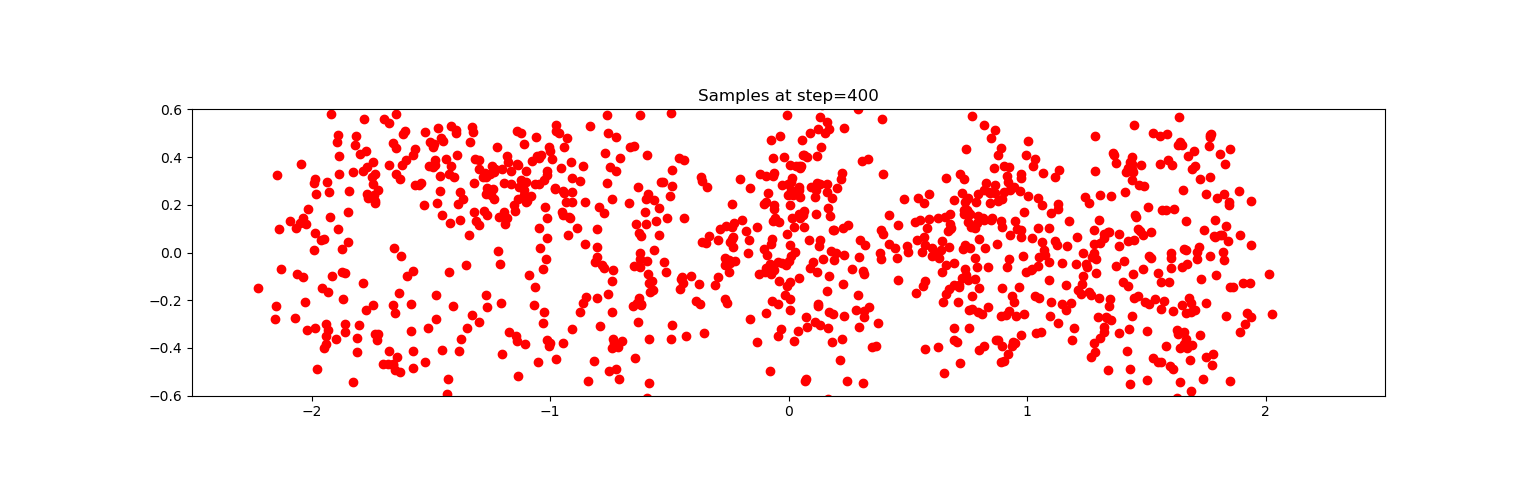
\includegraphics[width=\linewidth]{codes/imgs/diffusion/step400.png}
    \caption{Step 400}
    \label{fig:step400}
\end{figure}

\begin{figure}[H]
    \centering
    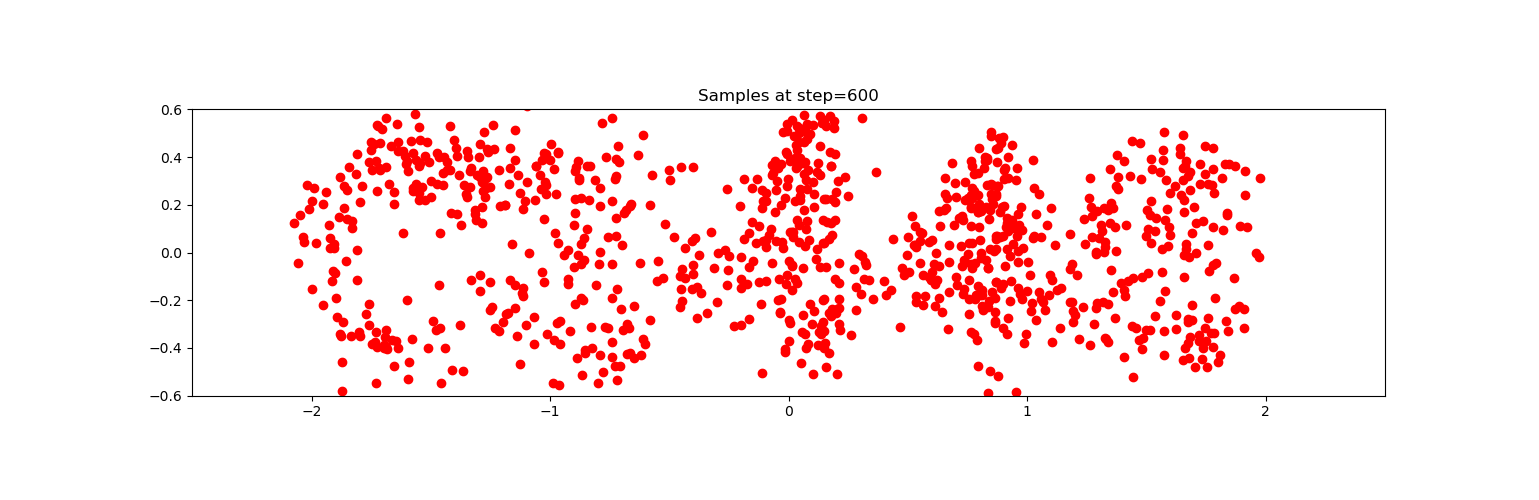
\includegraphics[width=\linewidth]{codes/imgs/diffusion/step600.png}
    \caption{Step 600}
    \label{fig:step600}
\end{figure}

\begin{figure}[H]
    \centering
    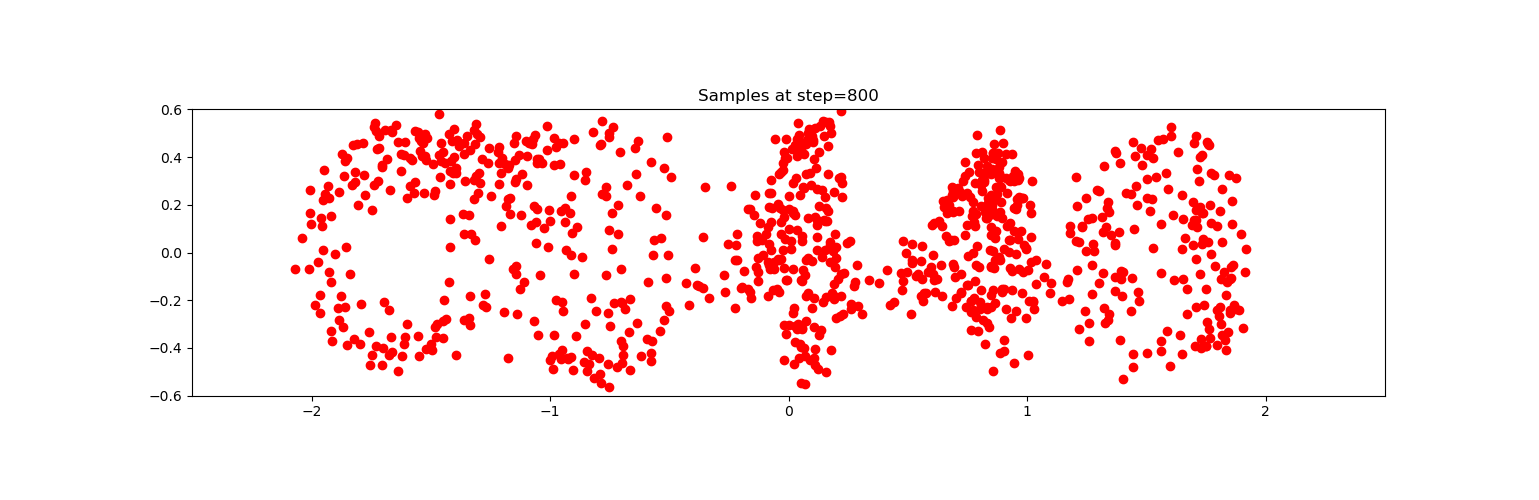
\includegraphics[width=\linewidth]{codes/imgs/diffusion/step800.png}
    \caption{Step 800}
    \label{fig:step800}
\end{figure}

\begin{figure}[H]
    \centering
    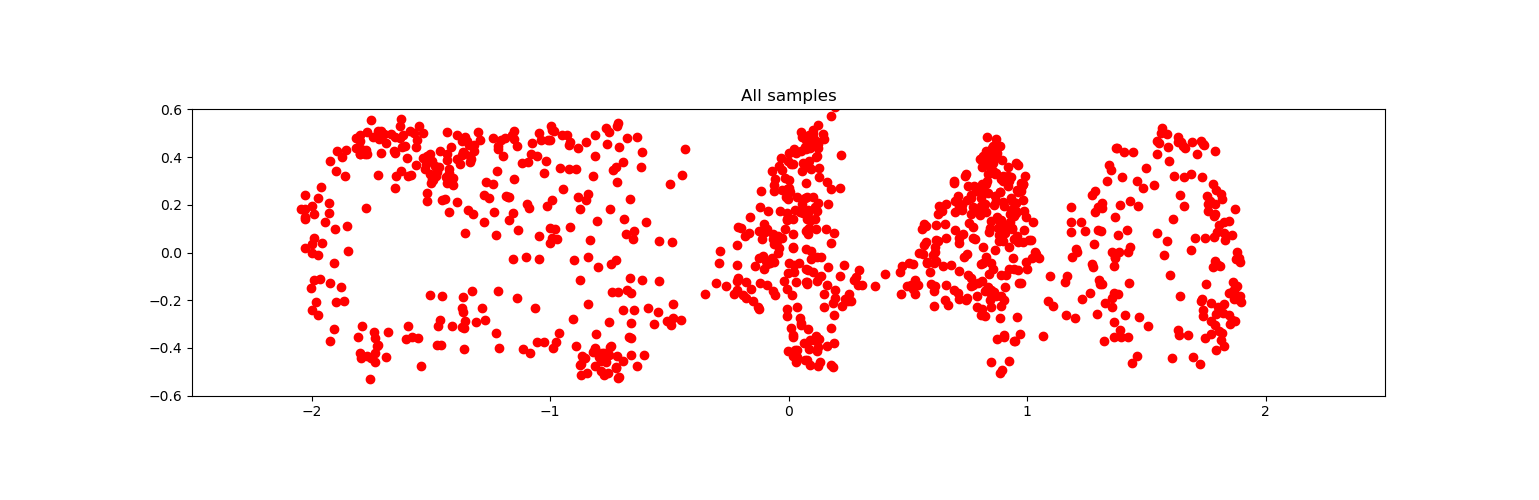
\includegraphics[width=\linewidth]{codes/imgs/diffusion/all.png}
    \caption{Final}
    \label{fig:step1000}
\end{figure}

\begin{figure}[H]
    \centering
    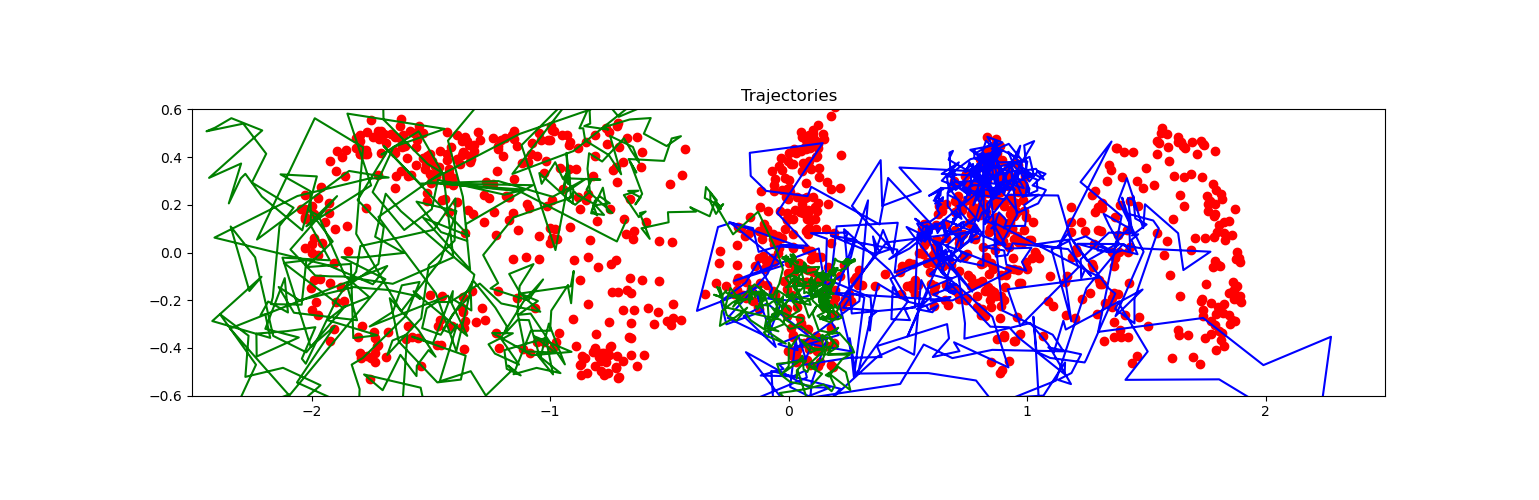
\includegraphics[width=\linewidth]{codes/imgs/diffusion/trajectory.png}
    \caption{Trajectory}
\end{figure}

\end{document}
